\section{Auswertung}
\label{sec:Auswertung}

\subsection{Statische Methode}
\label{sec:stat}

\begin{figure}
  \centering
  \includegraphics{T1_T4.pdf}
  \caption{Temperaturverlauf der Messingstäbe außen.}
  \label{fig:T1T4}
\end{figure}

\begin{figure}
  \centering
  \includegraphics{T5_T8.pdf}
  \caption{Temperaturverlauf von Aluminium und Edelstahl außen.}
  \label{fig:T5T8}
\end{figure}

\begin{figure}
  \centering
  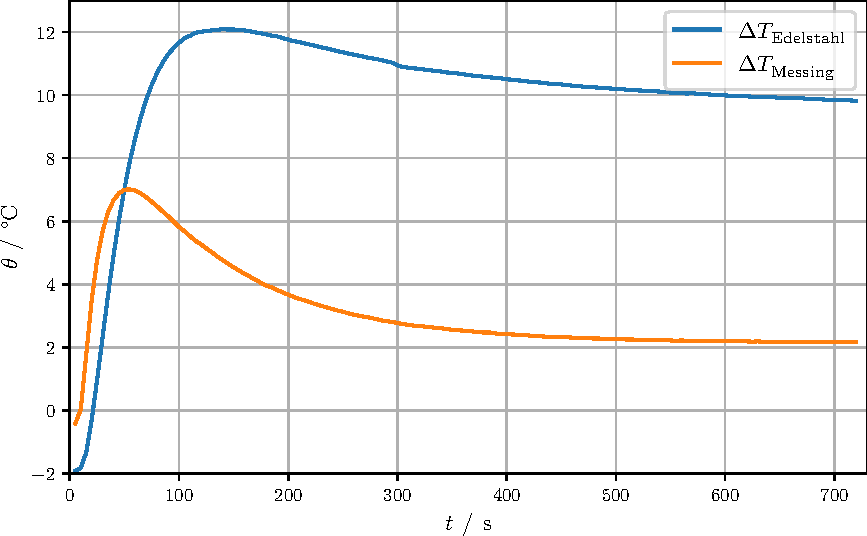
\includegraphics{Tempdiff.pdf}
  \caption{Temperaturdifferenz des breiten Messingstabs und des Edelstahlstabs.}
  \label{fig:Tempdiff}
\end{figure}

\subsection{Dynamische Methode}
\label{dynam}

\begin{figure}
  \centering
  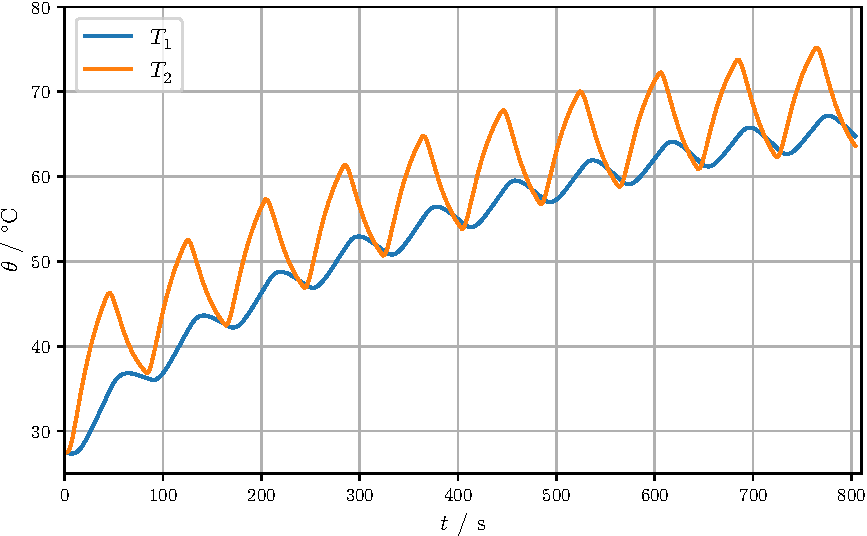
\includegraphics{80sMess.pdf}
  \caption{Temperaturverlauf des breiten Messingstabs.}
  \label{fig:80sMess}
\end{figure}

\begin{figure}
  \centering
  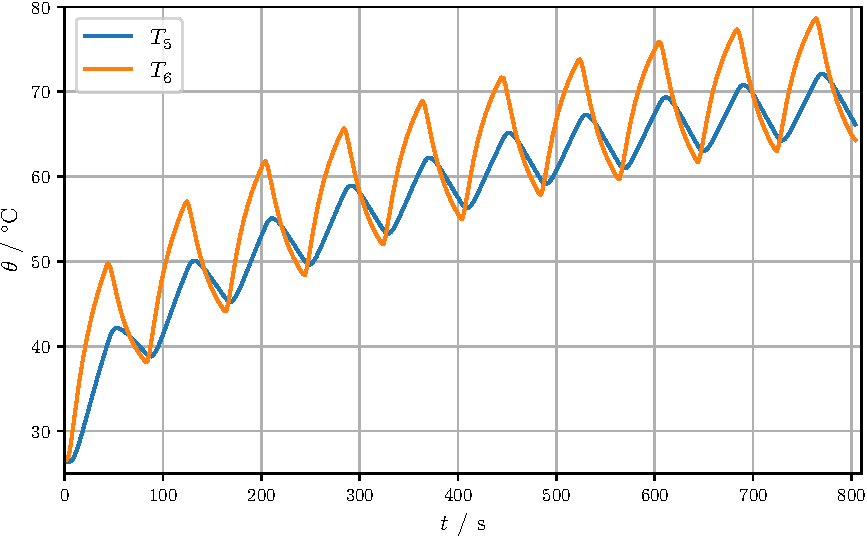
\includegraphics{80sAlu.pdf}
  \caption{Temperaturverlauf des Aluminiumstabs.}
  \label{fig:80sAlu}
\end{figure}

\begin{figure}
  \centering
  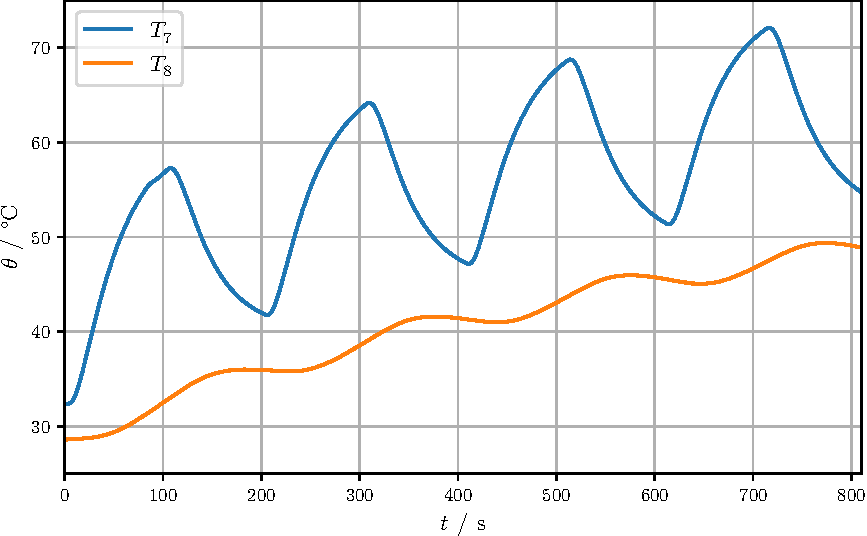
\includegraphics{200sEdelstahl.pdf}
  \caption{Temperaturverlauf des Edelstahlstabs.}
  \label{fig:200sEdelstahl}
\end{figure}
